\subsection{Сравнение одноэлектронных спектров при временном и амплитудном считывании}\label{section:secNxVsPadiwa}

%Первое предложение нужно изменить.
Как отмечено в секции~\ref{section:secMapmt}, у МА~ФЭУ H12700 имеются особенности, которые могут оказать влияние на эффективность регистрации единичных фотоэлектронов и вероятность возникновения ложных хитов. Для прояснения этих особенностей были выполнены измерения амплитудных распределений с помощью многоканальной платы на основе микросхемы n-XYTER, см. описание лабораторного стенда в секции~\ref{section:secLabSetup}. Далее, результаты амплитудных измерений были сопоставлены с данными, полученными с помощью платы PADIWA.

Амплитудные измерения с низким порогом продемонстрировали наличие заметного пика в малых амплитудах в спектре событий, скоррелированных с источником света.
%слишком длинное предложение
Специальные измерения с маской, открывающей только два разнесенных друг от друга на 2,5~см. пикселя, позволили установить, что событие с малой амплитудой в одном из каналов имеет место тогда, когда в другом канале, находящемся в том же ряду динодной системы, был зарегистрирован фотоэлектрон с достаточно большой амплитудой. Таким образом, для каналов с низкими шумами амплитудный спектр одноэлектронных сигналов выглядит как на рис.~\ref{fig:PeculiarSpectrum}.

\begin{figure}
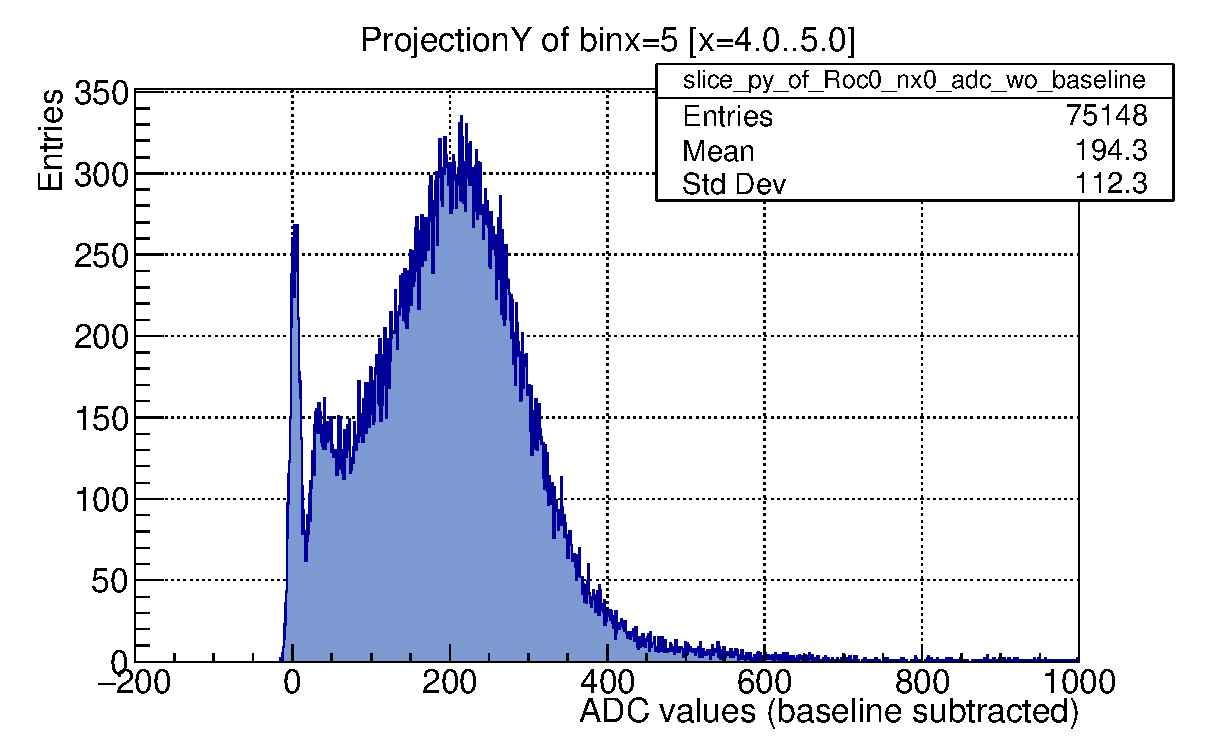
\includegraphics[width=1.0\textwidth]{pictures/PeculiarSpectrum.eps}
\caption{}
\label{fig:PeculiarSpectrum}
\end{figure}

Пик вблизи нуля соответствует наводке, возникающей в каналах, расположенных в одном ряду с тем, где зарегистрирован одноэлектронный сигнал. Двугорбое распределение справа соответствует настоящим одноэлектронным сигналам. Причем, левый пик связан с описанными в секции~\ref{section:secMapmt} событиями, когда электронная лавина или ее часть отклоняется от оптимального пути от динода к диноду. Отметим, что в большинстве каналов уровень шумов оказывается слишком высоким для отделения низкоамплитудного пика, связанного с наводкой от одноэлектронного сигнала. Таким образом, попытка получить максимальную эффективность регистрации за счет снижения порога приводит к возрастанию паразитных хитов, локализованных не в тех пикселях, где родился фотоэлектрон. Для снижения числа паразитных хитов мы ставили порог регистрации в ложбине между низко- и высоко-амплитудными частями одноэлектронного спектра. Поскольку формы одноэлектронных спектров во всех каналах подобны, анализ рисунка~\ref{fig:PeculiarSpectrum} позволяет заключить, что выбранный нами порог приводит к потере~???~\% одноэлектронных импульсов.

%пунктуация?
Одно из отличий канала считывания в плате PADIWA --- это значительно более быстрая, чем в n-XYTER аналоговая часть. Если в n-XYTER осуществляется формирование со временем интегрирования 190~нс, то в PADIWA происходит лишь подавление частот выше 100~МГц, что соответствует характерному времени нарастания сигнала несколько наносекунд. Такое отличие приводит к возрастанию роли быстрых шумов и наводок при регистрации сигналов с помощью PADIWA.

Информация о форме одноэлектронного спектра при считывании с помощью канала на основе плат PADIWA и TRB~v3 может быть получена в виде зависимости скорости счета событий вблизи триггера светового импульса от порога регистрации. Такие данные могут быть получены как из анализа потока даных, набранных при различных значениях порога, так и из значений счетчика зарегистрированых фронтов, реализованного непосредственно в ВЦП, упомянутого в секции~\ref{section:secModule}. При этом, использование счетчика позволяет достичь максимальных частот, достаточных для локализации базовой линии. На рис.~\ref{fig:TDCscalerScan} показана зависимость частоты триггеров в зависимости от порога регистрации. Плечо слева соответствует одноэлектронному спектру, а быстровозрастающие границы вблизи канала 34000 ограничивают локализацию базовой линии. Точность локализации базовой линии мы оцениваем как $ \pm $~??? отсчетов по шкале, использованной на рис.~\ref{fig:TDCscalerScan}.

%\begin{figure}
%\includegraphics[width=1.0\textwidth]{pictures/Thr_scan_flat.eps}
%\caption{Зависимость скорости счёта в одном канале от порога дискриминатора. Красная линия --- результат аппроксимации многочленом 7 степени.}
%\label{fig:ThrScan}
%\end{figure}

%\begin{figure}
%\includegraphics[width=1.0\textwidth]{pictures/Derivative_flat.eps}
%\caption{Аналитическая производная аппроксимирующей функции --- аналог одноэлектронного спектра.}
%\label{fig:ThrScanDeriv}
%\end{figure}

\begin{figure}
\includegraphics[width=1.0\textwidth]{pictures/TDCscalerScan.png}
\caption{}
\label{fig:TDCscalerScan}
\end{figure}

Результаты измерения частоты отсчетов, полученные с помощью счетчика и из анализа потока данных совпадают между собой, если полученное значение не превосходит *** при равномерной засветке всех каналов. (Совершенно не понятно, что это за предложение. Мы установили, что значения от этого счётчика совпадают со значениями, полученными анализом набранных данных. По-видимому, счётчик реально считает обработанные временные фронты, и если происходит затык из-за переизбытка фронтов, то и в данных и в счётчике будет спад, но одинаковый.)

Интересно сравнить зависимость скорости счета от порога при использовании двух систем считывания и одинаковых условиях засветки. Результаты такого сравнения для одного из типичных каналов показаны на рис.~\ref{fig:Blackboard}. В случае n-XYTER в таком сравнении может быть использован интеграл одноэлектонного спектра, показанный на рисунке~\ref{fig:Blackboard}a. Соответственно, производная указанной зависимости может быть сопоставлена с одноэлектронным спектром. Сплошная линия на рис.~\ref{fig:Blackboard}d получена дифференцированием кривой, показанной красным цветом на рис.~\ref{fig:Blackboard}b и полученной подгонкой измеренной зависимости полиномом 7-й степени. Отметим, что мы оцениваем равенство световых потоков как $ \pm $5\%. Видно, что скорости счета в области ложбины и максимума одноэлектронного спектра приблизительно совпадают. Амплитуды, соответствующие максимуму и ложбине соответственно, относятся как *** в обоих (или заметно отличие --- вряд ли, учитывая погрешность базовой линии!) случаях. При этом, в случае PADIWA наблюдается, с одной стороны более явно выраженная ложбина, а с другой --- избыток счета в малых амплитудах, что предполагает больший относительный вклад наводок и, следовательно, невозможность отделения от них низкоамплитудной части одноэлектронного спектра и нецелесообразность повышения эффективности за счет установления порога ниже ложбины.

\begin{figure}
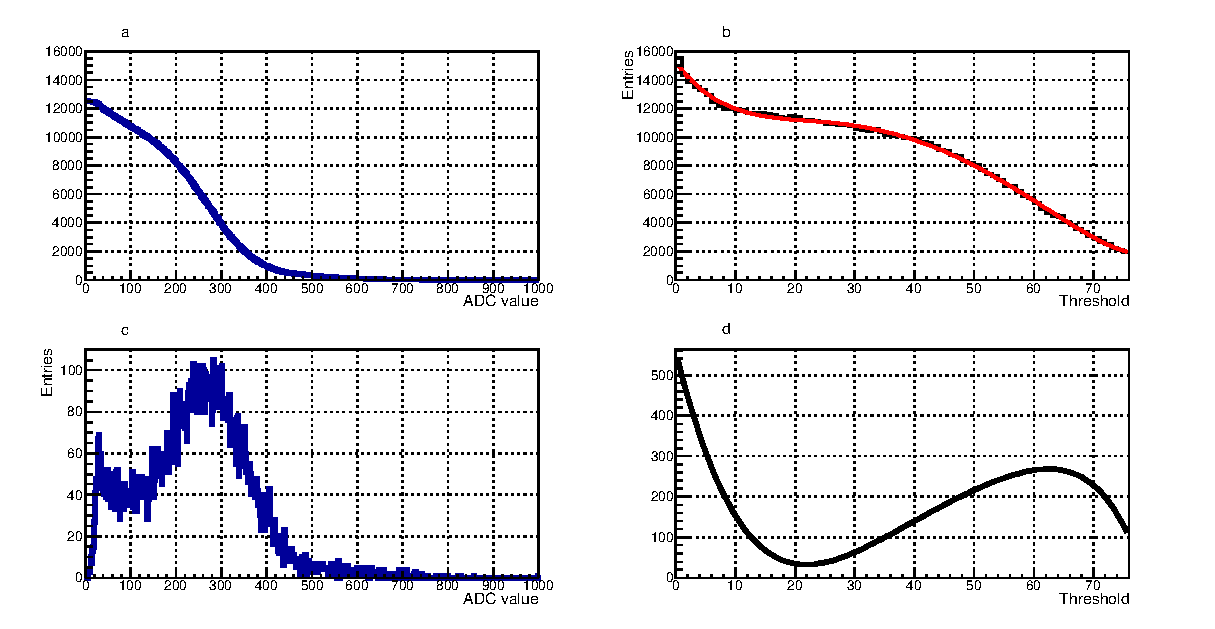
\includegraphics[width=1.0\textwidth]{pictures/Blackboard.eps}
\caption{}
\label{fig:Blackboard}
\end{figure}
